\documentclass[12pt, twoside]{article}
\usepackage[letterpaper, margin=1in, headsep=0.5in]{geometry}
\usepackage[english]{babel}
\usepackage[utf8]{inputenc}
\usepackage{amsmath}
\usepackage{amsfonts}
\usepackage{amssymb}
\usepackage{tikz}
\usetikzlibrary{quotes, angles}
\usepackage{graphicx}
\usepackage{enumitem}
\usepackage{multicol}

\newif\ifmeta
\metatrue %print standards and topics tags

\title{Regents Geometry}
\author{Chris Huson}
\date{September 2020}

\usepackage{fancyhdr}
\pagestyle{fancy}
\fancyhf{}
\renewcommand{\headrulewidth}{0pt} % disable the underline of the header
\raggedbottom


\fancyhead[LE]{\thepage}
\fancyhead[RO]{\thepage \\ Name: \hspace{4cm} \,\\}
\fancyhead[LO]{BECA / Dr. Huson / Geometry \\* 1-6 Angle measures}

\begin{document}

\subsubsection*{I can measure angles}
\begin{enumerate}
  \item Do Now: Given $\overline{LMN}$, $LM=3x+1$, $MN=7$, $LN=17$. Find ${x}$.\\[0.15in]
  \begin{tikzpicture}
   \draw [-, thick] (0,0)--(7,0);
   \draw [fill] (0,0) circle [radius=0.05] node[below]{$L$};
   \draw [fill] (4,0) circle [radius=0.05] node[below]{$M$};
   \draw [fill] (7,0) circle [radius=0.05] node[below]{$N$};
   \node at (1.7,0) [above]{$3x+1$};
   \node at (5.5,0) [above]{$7$};
   \draw [<->, dashed] (0,-1)--(7,-1);
   \node at (3.5,-1) [below]{$17$};
 \end{tikzpicture} %\vspace{1cm}
\begin{enumerate}
 \item Write down an equation to represent the situation. \vspace{0.5cm}
 \item Solve for $x$. \vspace{1.5cm}
 \item Check your answer. \vspace{1.5cm}
\end{enumerate}

\item Given an angle with vertex $A$.
  \begin{enumerate}[itemsep=0.5cm]
    \item Using a protractor, measure angle $A$ in degrees. $m\angle A =$
    \item Draw a ray $\overrightarrow{AB}$ that exactly bisects $\angle A$.
    \item What is the measure of each half angle?
  \end{enumerate}
  \begin{center}
  \begin{tikzpicture}
    \draw [<->, thick] (40:9)--(0,0)--(9,0);
    \draw [fill] (0,0) circle [radius=0.05] node[below]{$A$};
    %\draw [fill] (7,0) circle [radius=0.05] node[below]{$N$};
  \end{tikzpicture}
  \end{center}

\newpage
\subsubsection*{Angle measures using the Babylonian system of $360^\circ$ in a circle}
A full rotation is $360^\circ$ (a full ``turn'').\\[0.5cm]
A half turn (straight line) is $180^\circ$. \\[0.5cm]
$90^\circ$ is a quarter turn or a \emph{right} angle. \\[0.5cm]
\emph{Acute} angles measure less than $90^\circ$. \emph{Obtuse} angles measure more than $90^\circ$. \\[0.5cm]
\emph{Adjacent} angles (``next to'' each other) share a common ray and are external to each other. \vspace{0.2cm}

\item Write down the name of the \emph{three} angles shown in the diagram below and their angle measures, using your protractor. \vspace{1cm}
    \begin{center}
    \begin{tikzpicture}[scale=2]
      \draw [->, thick] (0,0)--(4,3);
      \draw [->, thick] (0,0)--(5,-.5);
      \draw [->, thick] (0,0)--(-1.2,3);
      \draw [fill] (-1,2.5) circle [radius=0.03] node[left ]{$B$};
      \draw [fill] (2.66666,2) circle [radius=0.03] node[above left ]{$C$};
      \draw [fill] (0,0) circle [radius=0.03] node[left]{$A$};
      \draw [fill] (4,-0.4) circle [radius=0.03] node[above]{$D$};
    \end{tikzpicture}
    \end{center}
    \begin{enumerate}
      \item  \rule{4cm}{0.15mm} \bigskip
      \item  \rule{4cm}{0.15mm} \bigskip
      \item  \rule{4cm}{0.15mm} \bigskip
      \item What do you notice about the angle measures?
    \end{enumerate}\vspace{1cm}

\item In your notebook, draw an angle that measures $55^\circ$

\newpage
\item 
\begin{enumerate}
  \item Write down the name of the angle shown in the diagram below using proper geometric notation.
  \item Find the measure of the angle in degrees with a protractor.
  \item Is it an acute, obtuse, or right angle?
\end{enumerate}
    \begin{flushright}
    \begin{tikzpicture}[scale=2]
      \draw [->, thick] (0,0)--(4,3);
      \draw [->, thick] (0,0)--(5,-1);
      \draw [fill] (2.66666,2) circle [radius=0.025] node[above left ]{$D$};
      \draw [fill] (0,0) circle [radius=0.025] node[above left]{$E$};
      \draw [fill] (4,-0.8) circle [radius=0.025] node[above]{$F$};
    \end{tikzpicture}
    \end{flushright}
    

\newpage    
\begin{center}
  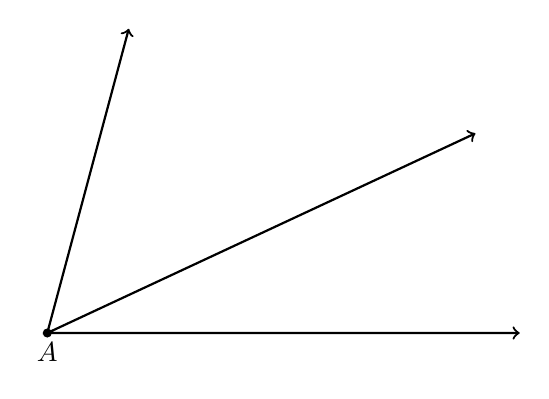
\begin{tikzpicture}
    \draw [<->, thick] (25:6)--(0,0)--(6,0);
    \draw [->, thick] (0,0)--(75:4);
    \draw [fill] (0,0) circle [radius=0.05] node[below]{$A$};
    %\draw [fill] (7,0) circle [radius=0.05] node[below]{$N$};
  \end{tikzpicture}
  \end{center}

\newpage
\item Given point $B$ is the midpoint of $\overline{AC}$, with $AB=x+2$, $BC=11$. \\[0.3cm]
    First write and equation representing the situation, then find $x$.\\[0.3cm]
      %\begin{center}
        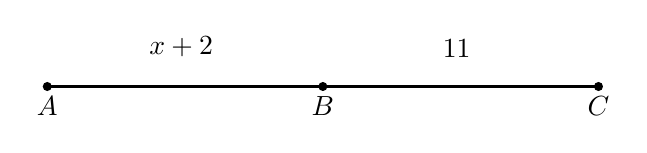
\begin{tikzpicture}
          \draw [fill] (0,0) circle [radius=0.05] node[below]{$A$};
          \draw [-, thick] (0,0)--(7,0);
          \draw [fill] (3.5,0) circle [radius=0.05] node[below]{$B$};
          \draw [fill] (7,0) circle [radius=0.05] node[below]{$C$};
          \node at (1.7,0.25) [above]{$x+2$};
          \node at (5.2,0.25) [above]{$11$};
          %\draw [<->, dashed] (0,-1)--(7,-1);
          %\node at (3.5,-1) [below]{$20$};
        \end{tikzpicture}
      %\end{center} 
      \vspace{1cm}

\item Find the value of each expression.
\begin{multicols}{2}
  \begin{enumerate}
    \item $|11|=$ \bigskip
    \item $|-7|=$
    \item $|-4.75|=$
    \item $|10-7|=$
  \end{enumerate}
\end{multicols} \vspace{0.5cm}

\item Given $\overleftrightarrow{QS}$ as shown on the number line. \\[20pt] % Midpoint
  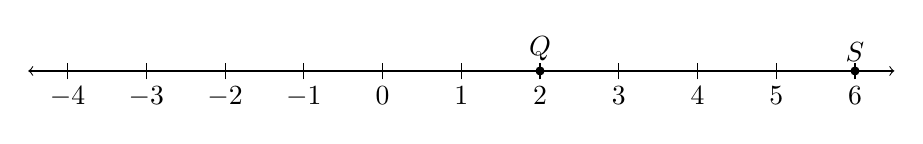
\begin{tikzpicture}
    \draw [<->] (-4.5,0)--(6.5,0);
    \foreach \x in {-4,...,6} %2 leading for diff!=1
      \draw[shift={(\x,0)},color=black] (0pt,-3pt) -- (0pt,3pt) node[below=5pt]  {$\x$};
      \draw [fill] (2,0) circle [radius=0.05] node[above] {$Q$};
      \draw [fill] (6,0) circle [radius=0.05] node[above] {$S$};
  \end{tikzpicture} \bigskip
  \begin{enumerate}
    \item In the given number line units, what is the distance between $Q$ and $S$? \\[0.5cm]
    $QS=$
    \bigskip
    \item Mark the point $R$, the midpoint of $\overline{QS}$.
  \end{enumerate}\vspace{1cm}

\item Given $\overline{MN}$ with $M(-1)$ and $N(3)$, as shown on the number line. \\[0.25cm]
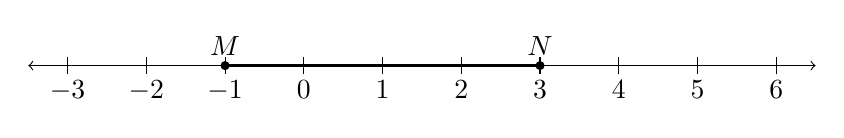
\begin{tikzpicture}
  \draw [<->] (-3.5,0)--(6.5,0);
  \draw [-, thick] (-1,0)--(3,0);
  \foreach \x in {-3,...,6} %2 leading for diff!=1
    \draw[shift={(\x,0)},color=black] (0pt,-3pt) -- (0pt,3pt) node[below=5pt]  {$\x$};
    \draw [fill] (-1,0) circle [radius=0.05] node[above] {$M$};
    \draw [fill] (3,0) circle [radius=0.05] node[above] {$N$};
\end{tikzpicture} \\ \bigskip
What is the length of the segment $\overline{MN}$? Show your work as an equation.
\end{enumerate}
\end{document}